% `template.tex', a bare-bones example employing the AIAA class.
%
% For a more advanced example that makes use of several third-party
% LaTeX packages, see `advanced_example.tex', but please read the
% Known Problems section of the users manual first.
%
% Typical processing for PostScript (PS) output:
%
%  latex template
%  latex template   (repeat as needed to resolve references)
%
%  xdvi template    (onscreen draft display)
%  dvips template   (postscript)
%  gv template.ps   (onscreen display)
%  lpr template.ps  (hardcopy)
%
% With the above, only Encapsulated PostScript (EPS) images can be used.
%
% Typical processing for Portable Document Format (PDF) output:
%
%  pdflatex template
%  pdflatex template      (repeat as needed to resolve references)
%
%  acroread template.pdf  (onscreen display)
%
% If you have EPS figures, you will need to use the epstopdf script
% to convert them to PDF because PDF is a limmited subset of EPS.
% pdflatex accepts a variety of other image formats such as JPG, TIF,
% PNG, and so forth -- check the documentation for your version.
%
% If you do *not* specify suffixes when using the graphicx package's
% \includegraphics command, latex and pdflatex will automatically select
% the appropriate figure format from those available.  This allows you
% to produce PS and PDF output from the same LaTeX source file.
%
% To generate a large format (e.g., 11"x17") PostScript copy for editing
% purposes, use
%
%  dvips -x 1467 -O -0.65in,0.85in -t tabloid template
%
% For further details and support, read the Users Manual, aiaa.pdf.


% Try to reduce the number of latex support calls from people who
% don't read the included documentation.
%


\typeout{}\typeout{If latex fails to find aiaa-tc, read the README file!}
%


\documentclass[]{aiaa-tc}% insert '[draft]' option to show overfull boxes
\usepackage{float}
\usepackage{epstopdf}
\usepackage{amsmath}
\usepackage[table,xcdraw]{xcolor}

\title{Zeus: Mission to Jupiter}

\author{
	Johnathan Clouse%
	\thanks{Graduate Student, Aerospace Engineering Sciences, 1111 Engineering Drive, Boulder, CO, 80309-0429}\\
	{\normalsize\itshape
		University of Colorado, Boulder, CO, 80309-0429, USA}
}

% Define commands to assure consistent treatment throughout document
\newcommand{\eqnref}[1]{(\ref{#1})}
\newcommand{\class}[1]{\texttt{#1}}
\newcommand{\package}[1]{\texttt{#1}}
\newcommand{\file}[1]{\texttt{#1}}
\newcommand{\BibTeX}{\textsc{Bib}\TeX}

\usepackage[euler]{textgreek}
\usepackage[colorlinks=true]{hyperref}
\hypersetup{urlcolor=cyan}

\usepackage{listings}
\usepackage{color} %red, green, blue, yellow, cyan, magenta, black, white
\definecolor{mygreen}{RGB}{28,172,0} % color values Red, Green, Blue
\definecolor{mylilas}{RGB}{170,55,241}

\usepackage{tablefootnote}
\usepackage{graphicx}
\usepackage{amsmath}
\usepackage{bm}
\usepackage{subfigure}
%\usepackage{subcaption}

\definecolor{mylilas}{RGB}{170,55,241}

% See p.105 of "TeX Unbound" for suggested values.
% See pp. 199-200 of Lamport's "LaTeX" book for details.
%   General parameters, for ALL pages:
\renewcommand{\topfraction}{0.9}	% max fraction of floats at top
\renewcommand{\bottomfraction}{0.8}	% max fraction of floats at bottom
%   Parameters for TEXT pages (not float pages):
\setcounter{topnumber}{2}
\setcounter{bottomnumber}{2}
\setcounter{totalnumber}{4}     % 2 may work better
\setcounter{dbltopnumber}{2}    % for 2-column pages
\renewcommand{\dbltopfraction}{0.9}	% fit big float above 2-col. text
\renewcommand{\textfraction}{0.07}	% allow minimal text w. figs
%   Parameters for FLOAT pages (not text pages):
\renewcommand{\floatpagefraction}{0.7}	% require fuller float pages
% N.B.: floatpagefraction MUST be less than topfraction !!
\renewcommand{\dblfloatpagefraction}{0.7}	% require
    \makeatletter
    \renewcommand\l@section{\@dottedtocline{2}{1.5em}{3em}}
    \makeatother
    
\begin{document}
	

	
	\maketitle
	
	\begin{abstract}
		\noindent 
		
	\end{abstract}
	
	\newpage
	
	\tableofcontents
	
	\newpage

	\section{Introduction}
Jupiter is the largest planet in the solar system, and the closest gas giant to the sun. It is a planet that is rich with opportunities for scientific inquiry. Jupiter's makeup can give clues to how the solar system was created. The largest moon, Ganymede, is thought to have a subsurface ocean and an active core. Europa also has a subsurface ocean, and geysers that spout water far above the surface. Either of these moons could hold life, but the first step in exploring them is to reach the Jupiter system.
	
	\vspace{5 mm}

A VEEGA (Venus-Earth-Earth Gravity Assist) trajectory for a mission called Zeus was considered for launch in 2020. The requirements are outlined as follows: time of flight fewer than ten years, C$_3$ under 18 km$^2$/s$^2$, arrival V$_\infty$ under 6 km/s, and total $\Delta$V$_\infty$ under 0.3 km/s for all gravity assists. The first step in finding a valid trajectory is to use Lambert's method to generate porkchop plots for all segments, except for resonant orbits, between planets. This will help the designer see what feasible trajectories exist, and whether each segment should be a Type I or Type II transfer. Next, an algorithm is applied to find one or more trajectories that meet the requirements. Finally, simulations can be performed using models of higher fidelity than the porkchop plots' Lambert solver. The designer can then correct the trajectory with propulsive maneuvers and determine overall feasibility of the orbit. 

	\section{Preliminary Trajectory Design}
The porkchop plots relevant to this trajectory are show in Figures \ref{fig:PCP_Launch_VGA}, \ref{fig:PCP_VGA_EGA1}, and \ref{fig:PCP_EGA2_JOI} below.
	\begin{figure}[H]
		\centering
			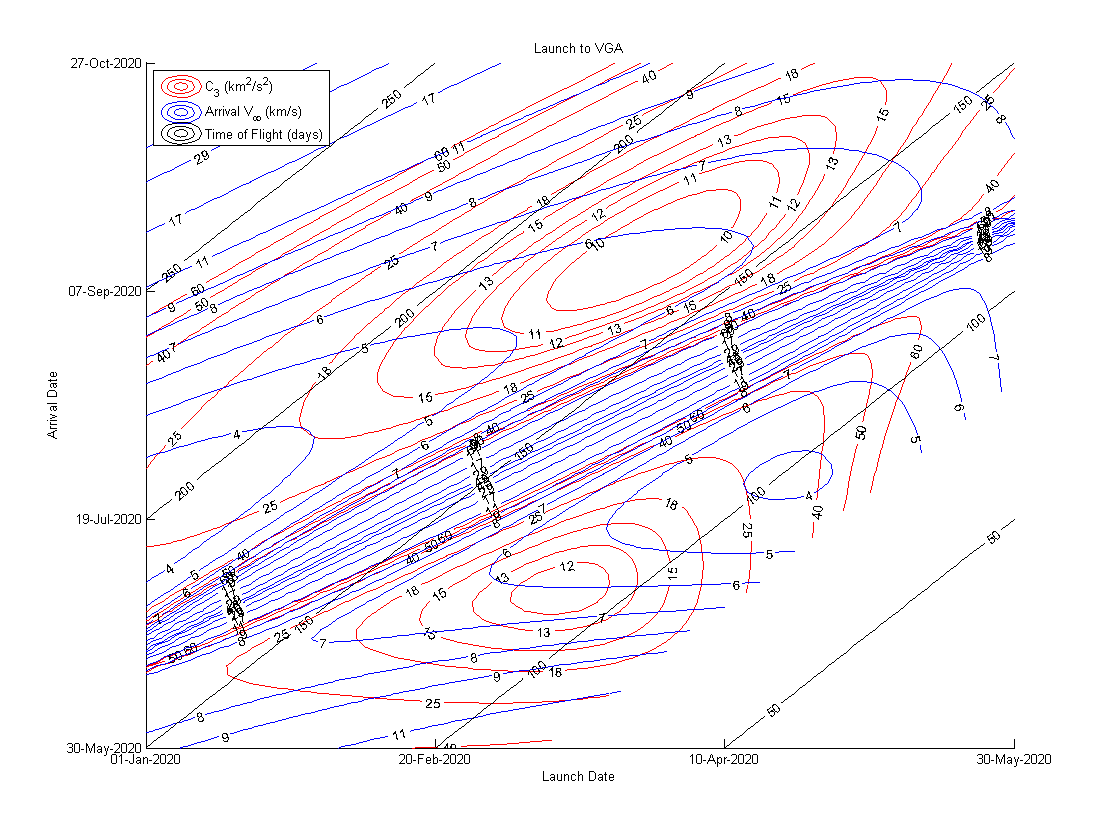
\includegraphics[width = 17.5cm]{../PCP/VEEJ/1_Launch_VGA.png}
		\caption{Launch to VGA. }
		\label{fig:PCP_Launch_VGA}
	\end{figure}	

	\begin{figure}[H]
		\centering
			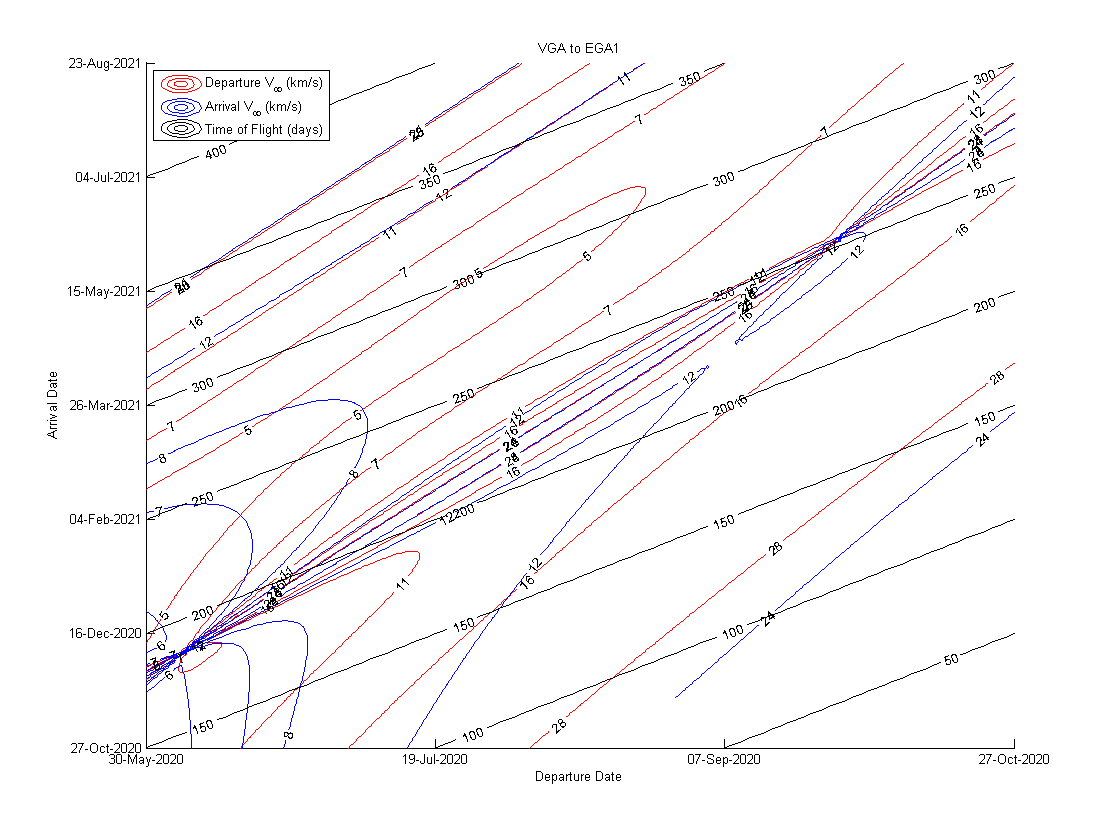
\includegraphics[width = 17.5cm]{../PCP/VEEJ/2_VGA_EGA1.png}
		\caption{VGA to EGA1. }
		\label{fig:PCP_VGA_EGA1}
	\end{figure}	

	\begin{figure}[H]
		\centering
			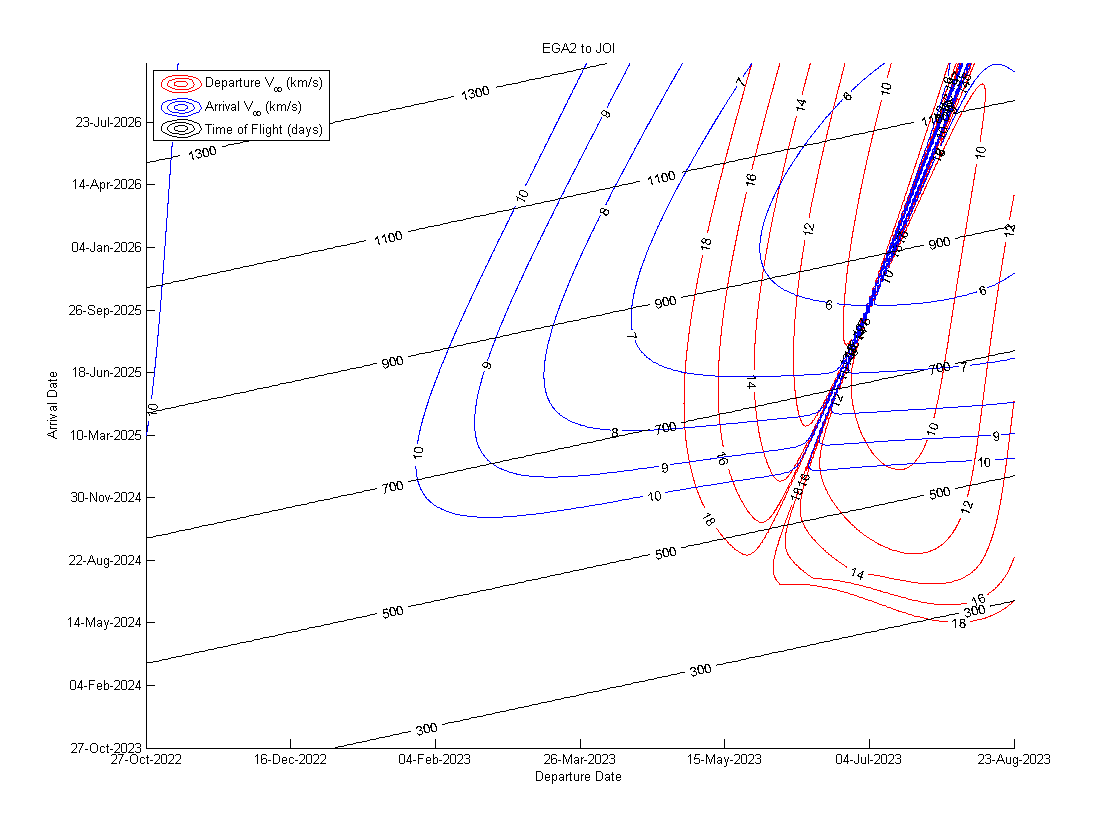
\includegraphics[width = 17.5cm]{../PCP/VEEJ/3_EGA2_JOI.png}
		\caption{EGA2 to JOI. }
		\label{fig:PCP_EGA2_JOI}
	\end{figure}	

From the above plots, one can see the dearth of planetary encounters that are supported with this launch date and the launch criteria. Type II transfers were chosen for the Earth-Venus and Venus-Earth segments, while a Type I transfer was chosen for the Earth-Jupiter segment. Other planetary encounter windows were tried for a 2020 launch date, but none were found.
	
	\vspace{5 mm}

	Porkchop plots serve as great visual guides to determine low-cost trajectories. However, chaining together multiple gravity assists leads to many potential solutions whose benefits become difficult to compare using several porkchop plots. An algorithm was developed to trim the search space of the possible trajectories, as well as to determine the merits of each trajectory. The algorithm took a predetermined set of windows and determined the Lambert solution between the launch, gravity assists, and orbit insertion. Next, launch C3 and final $V_\infty$ were applied to the initial and final windows to rid the search space of known unusable trajectories. The ${\Delta}V$ difference between planetary encounters on a given date were subsequently calculated; any ${\Delta}V$ difference outside of a tuned tolerance were thrown out. The result was a set of dates that fit the given requirements. The space was further pruned by calculating the closest approach to all flyby planets and discarding the ones that got too close.
	
	\vspace{5 mm}

	Performance of this algorithm was found to be very hardware-dependent. The algorithm was implemented in Matlab and run on a 6-year-old desktop computer. For the VEEGA trajectory to Jupiter, the process took over 40 minutes to reach the point of calculating the closest approach for all the flybys. The same algorithm and data run on a computer with 16 cores and 64 GB of RAM did the entire algorithm in under five minutes. No doubt this hardware could find valid trajectory to the ice giants with smaller granularity in the encounter windows, but its availability was late-coming.
	
	\vspace{5 mm}

Dates were chosen to minimize the V$_\infty$ errors in the calculated gravity assist. Table \ref{TrajParams} shows the chosen dates and the relevant targeting parameters.
% Please add the following required packages to your document preamble:
% \usepackage[table,xcdraw]{xcolor}
% If you use beamer only pass "xcolor=table" option, i.e. \documentclass[xcolor=table]{beamer}
\begin{table}[H]
\centering
\caption{Trajectory parameters}
\label{TrajParams}
\begin{tabular}{|c|c|c|l|}
\hline
\rowcolor[HTML]{C0C0C0} 
\textbf{Event}                                                           & \textbf{Calendar Date}                                                & \textbf{Julian Date} & \multicolumn{1}{c|}{\cellcolor[HTML]{C0C0C0}\textbf{Information}}                      \\ \hline
Launch                                                                   & \begin{tabular}[c]{@{}c@{}}25 February 2020 \\ 12:52:48\end{tabular}  &          2458906            & \begin{tabular}[c]{@{}l@{}}C$_3$: 16.72 $\mathrm{km^2/s^2}$\\ RLA: 108.64$^\circ$\\ DLA: 7.52$^\circ$\\ Launched from \\ Tanegashima, Japan\end{tabular} \\ \hline
\begin{tabular}[c]{@{}c@{}}Venus Gravity Assist \\ (VGA)\end{tabular}    & \begin{tabular}[c]{@{}c@{}}15 September 2020 \\ 12:00:00\end{tabular} &                     2459108 & \begin{tabular}[c]{@{}l@{}}r$_\mathrm{p}$: 23224 km\\ B$_\mathrm{T}$: 29790\\ B$_\mathrm{R}$: 4735.7\\ Turning Angle: 29.63$^\circ$ \\ V$_\infty$: 6.39 km/s\\$\Delta$V$_\infty$: 2.7298e-4 km/s\end{tabular}                           \\ \hline
\begin{tabular}[c]{@{}c@{}}Resonant Orbit\end{tabular} &  -- & -- & \begin{tabular}[c]{@{}l@{}}Resonance: 2:1 \\$\varphi$: 130.06$^\circ$ \\ V$_\infty$: 9.45 km/s\\$\Delta$V$_\infty$: 2.7298e-4 km/s\end{tabular}                           \\ \hline
\begin{tabular}[c]{@{}c@{}}Earth Gravity Assist 1 \\ (EGA1)\end{tabular} & \begin{tabular}[c]{@{}c@{}}12 July 2021 \\ 12:00:00\end{tabular}      &           2459408           & \begin{tabular}[c]{@{}l@{}}r$_\mathrm{p}$: 6745.2 km\\ B$_\mathrm{T}$: -7069.2 km\\ B$_\mathrm{R}$: -7474.7 km\\ Turning Angle: 47.00$^\circ$ \end{tabular}                           \\ \hline
\begin{tabular}[c]{@{}c@{}}Earth Gravity Assist 2 \\ (EGA2)\end{tabular} & \begin{tabular}[c]{@{}c@{}}12 July 2023 \\ 12:00:00\end{tabular}      &         2460138             & \begin{tabular}[c]{@{}l@{}}r$_\mathrm{p}$: 7079.5 km\\ B$_\mathrm{T}$:-10549 km\\ B$_\mathrm{R}$: 1472.1 km\\ Turning Angle: 45.56$^\circ$ \end{tabular}                           \\ \hline
\begin{tabular}[c]{@{}c@{}}Jupiter Orbit Insertion \\ (JOI)\end{tabular} & \begin{tabular}[c]{@{}c@{}}14 February 2026 \\ 12:00:00\end{tabular}  &                     2461086 & \begin{tabular}[c]{@{}l@{}}V$_\infty$: 5.5868 km/s\\ $\Delta$V: 1.5336 km/s\\$\left |{\vec{B}}  \right |$: 3.1108e6 km\\ Inclination: 0$^\circ$\\ r$_\mathrm{p}$: 1.0711e6 km\\ r$_\mathrm{a}$: 1.4707e7 km\\ Period: 143.1 days\end{tabular}             \\ \hline
\end{tabular}
\end{table}

As Table \ref{TrajParams} shows, the $\Delta$V$_\infty$ is quite low for each gravity assist. The resonant orbit gravity assist's $\Delta$V$_\infty$ is the error between the initial approach and final departure; the V$_\infty$ magnitude between these times is assumed to be within this error. Because the errors were non-zero, trajectory correction maneuvers (TCM) will have to be performed to allow the spacecraft to reach the calculated B-plane targets. The flyby altitude for each planet is greater than 300 km. Not only does this prevent planetary impact, it reduces drag that a TCM would have to correct. With Earth encounters, conjunction analysis should be performed to ensure there is no risk to hitting another spacecraft. In addition, one must ensure that the Moon does not interfere with or stand in the way of the trajectory. TCMs will have to account for lunar perturbations.
	
	\vspace{5 mm}

The resonant orbit periapses are shown in Figure \ref{fig:reso} below.
	\begin{figure}[H]
		\centering
			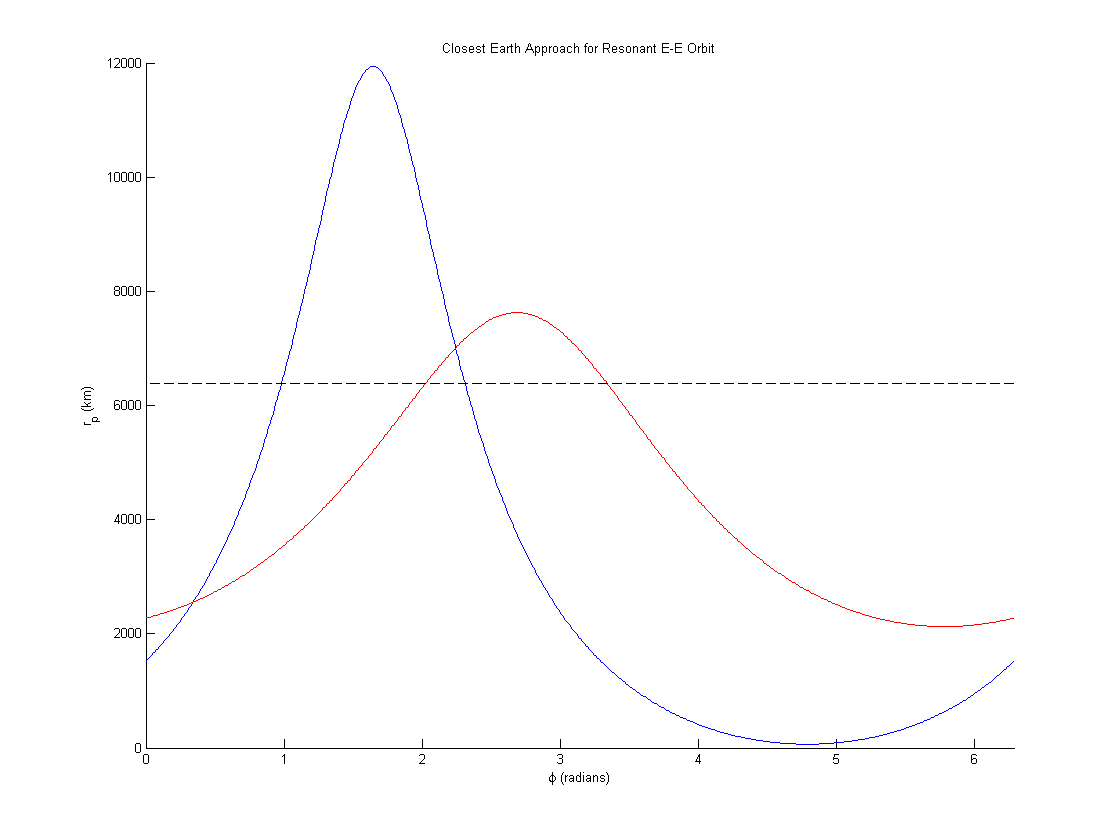
\includegraphics[width = 18cm]{../PCP/VEEJ/PhiVsRp.png}
		\caption{Resonant orbit periapses. }
		\label{fig:reso}
	\end{figure}	

The range of $\varphi$ that prevents planetary impact for both gravity assists is small. The value of $\varphi$ was chosen approximately where the periapses are the same (and greater than the radius of Earth) to ensure minimum drag effects on both flybys. 
	
	\vspace{5 mm}

Jupiter's moons can provide both scientific targets and gravity assists. Ganymede, being the most massive body, has been identified as the most useful Jovian moon for changing the spacecraft period\cite{Damario}. This moon is outside the worst of Jupiter's radiation, making its orbit safe for spacecraft perijove. Ganymede's orbital radius is 1.0711e6 km in radius from Jupiter with an eccentricity of 0.001\cite{Damario}. Choosing a 20:1 resonant initial orbit with Ganymede gave the spacecraft an apojove of 1.4707e7 km and period of 143.1 days, requiring a JOI $\Delta$V of 1.5336 km/s. Larger initial orbits substantially increased the period while encountering diminishing returns with the JOI $\Delta$V. This initial orbit could allow for a varietry of moon tours that would lower apojove and allow easier capture around one of the moons. In addition, the outer Galilean moons could reduce the JOI burn required. For this trajectory, Ganamede could provide a turning angle of up to 11$^\circ$. To find the magnitude of $\vec{B}$, one merely computes the hyperbola equation $b=a\sqrt{e^2-1}$ to find that $\left |{\vec{B}}  \right |= b = $ 3.1108e6 km.
	
	\vspace{5 mm}

A Hohmann transfer from Earth to Jupiter was constructed using semimajor axes of the planets given by Vallado\cite{Vallado} and assuming circular planetary orbits. It is shown alongside the trajectory requirements and the actual performance in Table \ref{TrajReqs} below. 
\begin{table}[H]
\centering
\caption{Trajectory requirements}
\label{TrajReqs}
\begin{tabular}{|c|c|c|c|}
\hline
\rowcolor[HTML]{C0C0C0} 
\textbf{Parameter}     & \textbf{Requirement} & \textbf{Actual}& \textbf{Hohmann} \\ \hline
Time of flight (years) & \textless10          & 6       & 2.7        \\ \hline
C3 ($\mathrm{km^2/s^2}$)              & \textless18          & 16.72     & 77.31      \\ \hline
Arrival V$_\infty$ (km/s)       & \textless6           & 5.59       & 5.64     \\ \hline
Total $\Delta$V$_\infty$ (km/s)         & \textless0.3           & 2.65e-4    & N/A     \\ \hline
\end{tabular}
\end{table}
The Hohmann transfer to Jupiter looked attractive due to the shorter time of flight, but the C$_3$ is prohibitively large. In fact, it's off the chart given by Vallado\cite{Vallado}. The proposed trajectory is most easily compared to the Galileo mission. Galileo was flown to study Jupiter and its moons; one could surmise that the mass of the spacecraft would be comparable. Like the proposed trajectory, Galileo took advantage of a VEEGA. Galileo's time of flight was just over six years. It also had a maximum C$_3$ of 17 $\mathrm{km^2/s^2}$\cite{Damario}. With a V$_\infty$ error orders of magnitude less than the maximum allowable, this trajectory was determined to be feasible. The primary difference between this trajectory and Galileo's was its JOI $\Delta$V of 0.630 km/s.  Galileo flew by Europa and Io to reduce its Jupiter-centric velocity. As previously  discussed, moon flybys could reduce the JOI $\Delta$V required by this trajectory.

	\section{STK Simulation}
The previously documented trajectory was visualized in STK 10. STK allows for simulations of spacecraft and ground facilities to give mission planners much of what they need to detail the spacecraft operations. It computes access between spacecraft and facilities. With the Astrogator package, STK assists in targeting interplanetary trajectories. It can take a savvy mission designer to know the best ways to target a trajectory, but the visualization and reports make communication to spacecraft designers easy. However, STK lacks the ability to search for trajectories given the requirements for this project. Therefore, one must create a trajectory in a similar fashion as described above. STK does allow for custom plugins, which could allow the STK application to be more capable in targeting trajectories. 
	
	\vspace{5 mm}

Planetary ephemerides were from DE421. Launch was originally targeted at Cape Canaveral, but there was difficulty in targeting the desired launch declination. Baikonur was the second choice, but the launch intersected Earth on its way out. Tanegashima successfully launched the spacecraft. Tanegashima is 2$^\circ$ above Cape Canaveral, so they are relatively similar for launch purposes.  Tanegashima can host interplanetary-bound spacecraft, but assuming Zeus is an American mission, there are regulatory constraints to launch from there.
	
	\vspace{5 mm}

TCMs were targeted 10 days after each planetary flyby. This time period was found to be far enough from the previous planetary encounter that third-body effects would be small in the overall propagation. Being quite early in the segment, TCM $\Delta$V was kept low. The TCMs are outlined in Table \ref{TCMTable} below.

\begin{table}[H]
\centering
\caption{STK Trajectory Correction Maneuvers}
\label{TCMTable}
\begin{tabular}{|c|c|c|c|}
\hline
\rowcolor[HTML]{C0C0C0} 
\textbf{Maneuver} & \textbf{Calendar Date}                                                   & \textbf{Julian Date} & \textbf{$\Delta$V (km/s)} \\ \hline
TCM1              & \begin{tabular}[c]{@{}c@{}}6 Mar 2020 \\ 15:18:46.684 UTCG\end{tabular}  & 2458915.13804032     & 0.1042                 \\ \hline
TCM2              & \begin{tabular}[c]{@{}c@{}}25 Sep 2020 \\ 11:59:59.979 UTCG\end{tabular} & 2459117.99999976     & 0.1309                 \\ \hline
TCM3              & \begin{tabular}[c]{@{}c@{}}22 Jul 2021 \\ 12:00:00.012 UTCG\end{tabular} & 2459418.00000013     & 0.3551                 \\ \hline
TCM4              & \begin{tabular}[c]{@{}c@{}}22 Jul 2023 \\ 12:00:00.000 UTCG\end{tabular} & 2460148              & 1.0372                 \\ \hline
\end{tabular}
\end{table}

The TCMs start small, but TCM4 ends up being quite large. This is due in part to the ephemerides being used in the Lambert solution (Meeus\cite{Meeus}) versus in STK (DE421). The initial TCMs have smaller adjustments to make due to the time and distance scales being small. TCM4 corrects a segment that goes much farther and takes more time, enhancing the error between the ephemerides. The Lambert solution assumed simple two-body motion, whereas STK's heliocentric propagator includes the gravity effects from all the planets. The TCMs could be smaller if the Lambert solver and STK ephemerides were the same. In addition, a smaller-granularity Lambert solution window for all planetary encounters could allow for better planetary targeting.
	
	\vspace{5 mm}

The trajectory has been visualized in Figures \ref{fig:InnerTrajectory} and \ref{fig:OuterTrajectory} below.
	\begin{figure}[H]
		\centering
		\subfigure[Above Ecliptic]{
			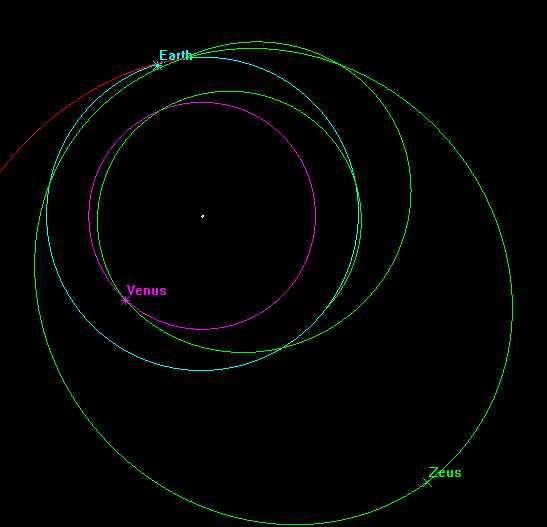
\includegraphics[width = 8cm]{../Figures/InnerTrajAbove.png}
		}
		\subfigure[Side view]{
			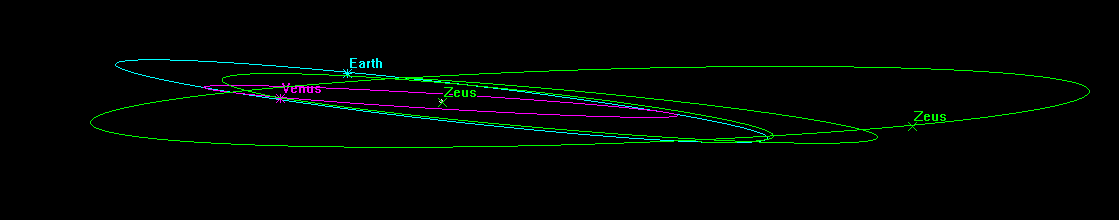
\includegraphics[width = 8cm]{../Figures/InnerTrajSunEquatorial.png}
		}
		\caption{Inner Trajectory. }
		\label{fig:InnerTrajectory}
	\end{figure}	
	\begin{figure}[H]
		\centering
		\subfigure[Above Ecliptic]{
			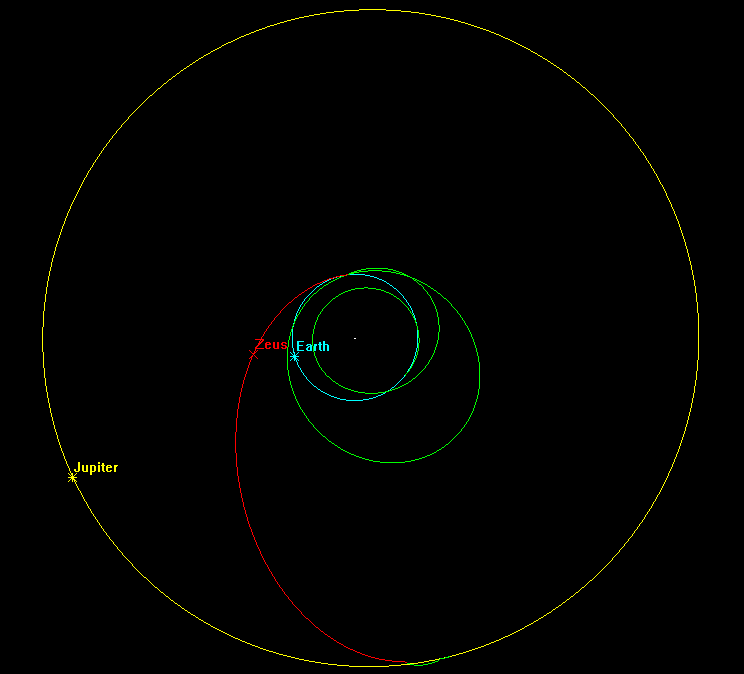
\includegraphics[width = 8cm]{../Figures/OuterTrajAbove.png}
		}
		\subfigure[Side view]{
			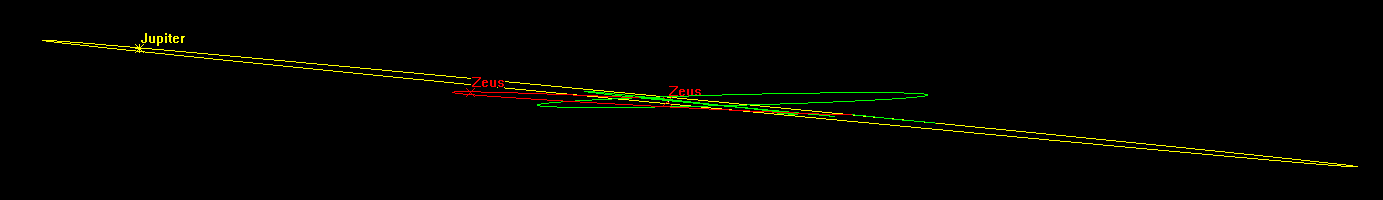
\includegraphics[width = 8cm]{../Figures/OuterTrajSunEquatorial.png}
		}
		\caption{Outer Trajectory. }
		\label{fig:OuterTrajectory}
	\end{figure}	

The STK-visualized trajectory looks as expected. There is a Type II trajectory from Earth to Venus, Type II from Venus to Earth, a resonant orbit that goes beyond Earth's, and a Type I trajectory to Jupiter. The trajectory from Earth to Jupiter almost looks like a Hohmann transfer, but with a significantly less launch C$_3$. The JOI and initial Jupiter orbit can be seen in Figure \ref{fig:JOI} below.

	\begin{figure}[H]
		\centering
			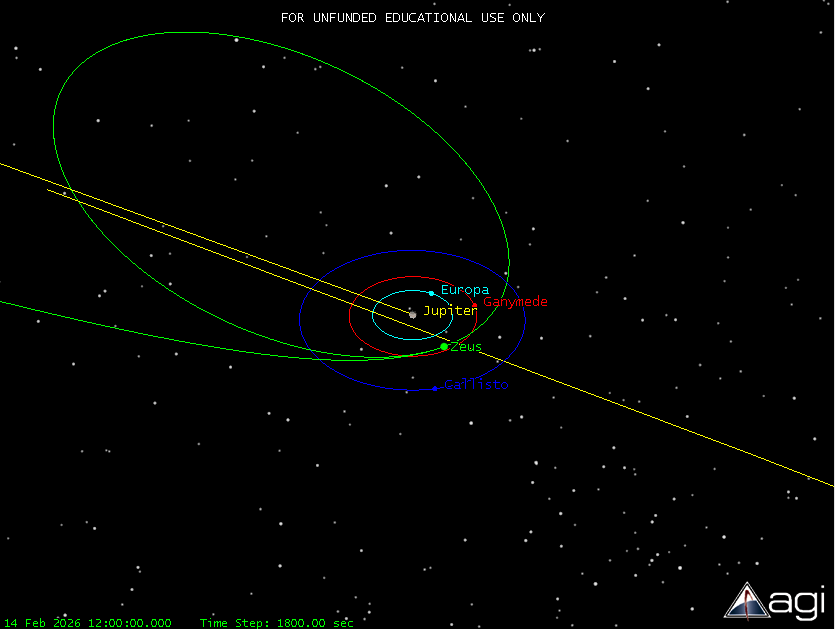
\includegraphics[width = 18cm]{../Figures/JOI_Initial_orb.png}
		\caption{JOI and initial orbit. }
		\label{fig:JOI}
	\end{figure}	

The B-plane target was chosen to be the $\left |{\vec{B}}  \right |$ found in the trajectory design, applied entirely in $+\hat{T}$. A positive value of $\hat{T}$ was necessary for prograde motion around Jupiter, since its tilt with respect to the ecliptic plane is small. This resulted in a small inclination (2$^\circ$) and a period of 142.33 days. The orbit intersects with Ganymede, which will allow for apojove-lowering maneuvers.

	\section{Earth Access}

Earthly access to a spacecraft is an important aspect of the mission. Software can be uploaded, commands sent, telemetry received, and emergencies abated as long as a ground station and the spacecraft have an unobstructed view of one another. It is desirable to see the spacecraft during maneuvers for navigation purposes so that the resulting state can be reconstructed. Figure \ref{fig:week1AccessGT} shows the ground track during the first week of the mission, along with the Deep Space Network (DSN) ground stations.
	\begin{figure}[H]
		\centering
			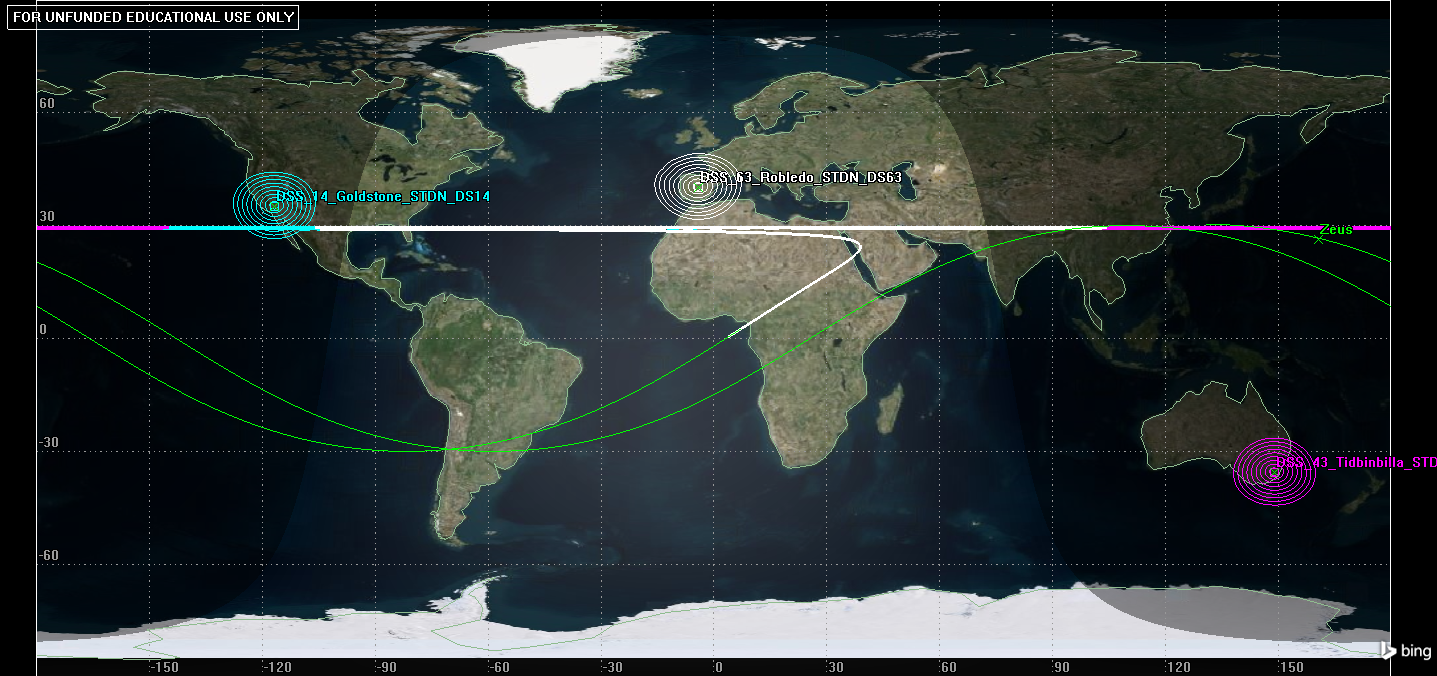
\includegraphics[width = 12cm]{../Figures/Week1GroundTrack.png}
		\caption{Week 1 ground track. }
		\label{fig:week1AccessGT}
	\end{figure}	

The spacecraft is visible from the Madrid facility during launch injection, ascertained by the white access line on the ground track. As the craft leaves the earth, it has retrograde motion on the ground track. The first week of DSN access can be seen in Figure \ref{fig:week1Access}.
	\begin{figure}[H]
		\centering
			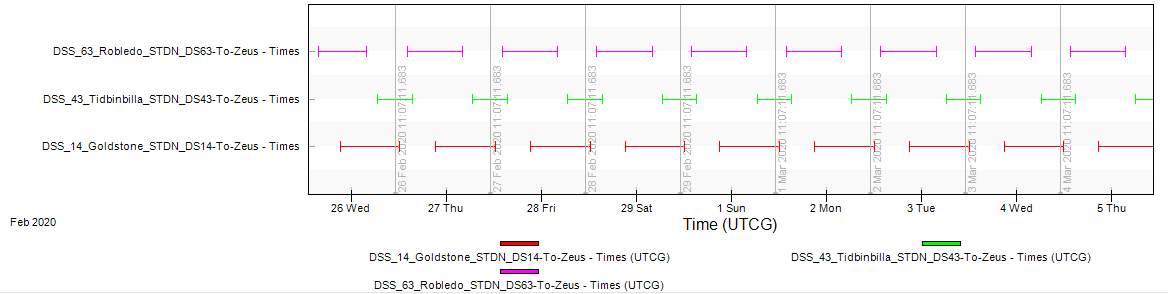
\includegraphics[width = 18cm]{../Figures/Week1Access.png}
		\caption{Week 1 DSN access. }
		\label{fig:week1Access}
	\end{figure}	

 The spacecraft is visible to the DSN with at least one station for the rest of the week. Sometimes there is double-coverage available by the facilities.

	\vspace{5 mm}

The Venus gravity assist DSN access is visualized in Figure \ref{fig:VGA_Access}.
	\begin{figure}[H]
		\centering
		\subfigure[VGA as seen from Earth]{
			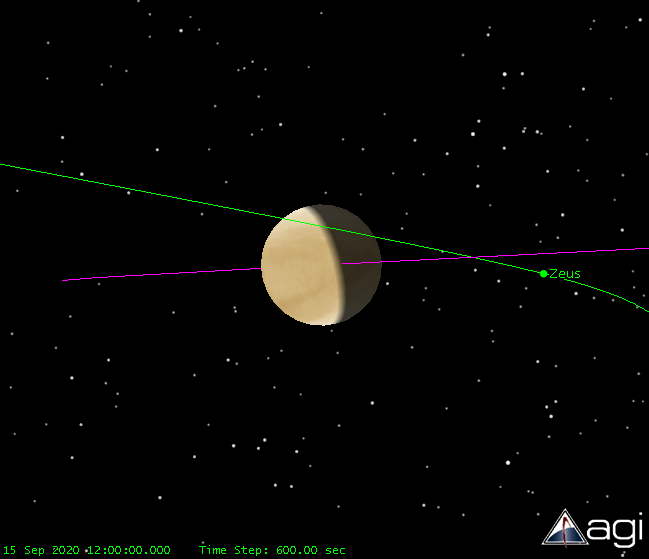
\includegraphics[width = 10cm]{../Figures/VGA_From_Earth.png}
		}
		\subfigure[VGA DSN access]{
			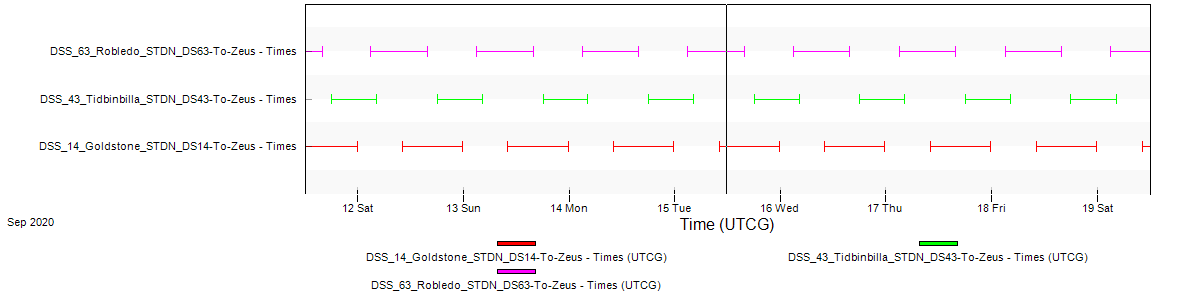
\includegraphics[width = 17cm]{../Figures/VGA_Access.png}
		}
		\caption{VGA visibility to the DSN. }
		\label{fig:VGA_Access}
	\end{figure}	

The VGA is most visible from Madrid. One could note that even if Venus obstructed the spacecraft view during closes approach, the spacecraft would be visible quite soon after. In fact, the access scenario is worst-case when the sun is in conjunction with the maneuver. A mission planner should take this into account when designing gravity assists, as there could be adverse impacts on the navigation solution if the maneuver wasn't executed as planned.

	\vspace{5 mm}

The first Earth gravity assist's DSN access is visualized in Figure \ref{fig:EGA1_Access}.
	\begin{figure}[H]
		\centering
		\subfigure[EGA1 closest approach]{
			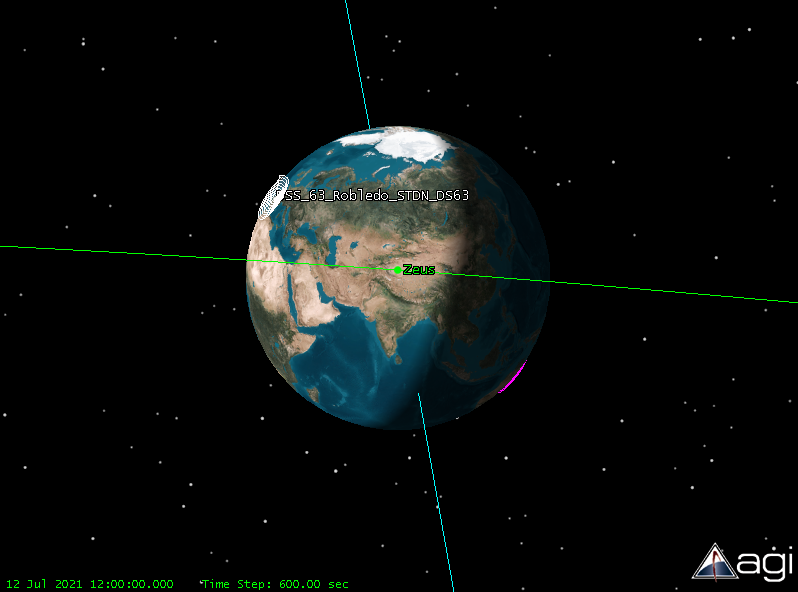
\includegraphics[width = 10cm]{../Figures/EGA1_3d.png}
		}
		\subfigure[EGA1 DSN access]{
			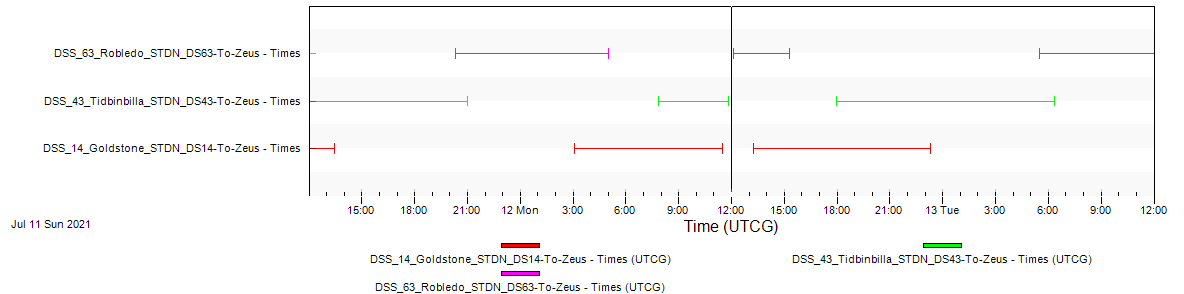
\includegraphics[width = 17cm]{../Figures/EGA1_Access.png}
		}
		\caption{EGA1 visibility to the DSN. }
		\label{fig:EGA1_Access}
	\end{figure}	
EGA1 is not visible at the closest approach. However, there are long access periods immediately before and after the maneuver. 

	\vspace{5 mm}

The second Earth gravity assist's DSN access is visualized in Figure \ref{fig:EGA2_Access}.
	\begin{figure}[H]
		\centering
		\subfigure[EGA2 closest approach]{
			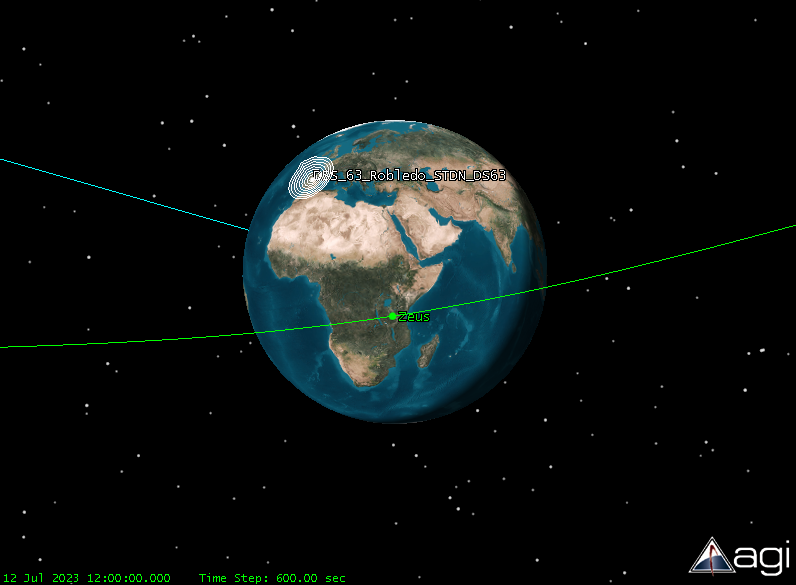
\includegraphics[width = 10cm]{../Figures/EGA2_3d.png}
		}
		\subfigure[EGA2 DSN access]{
			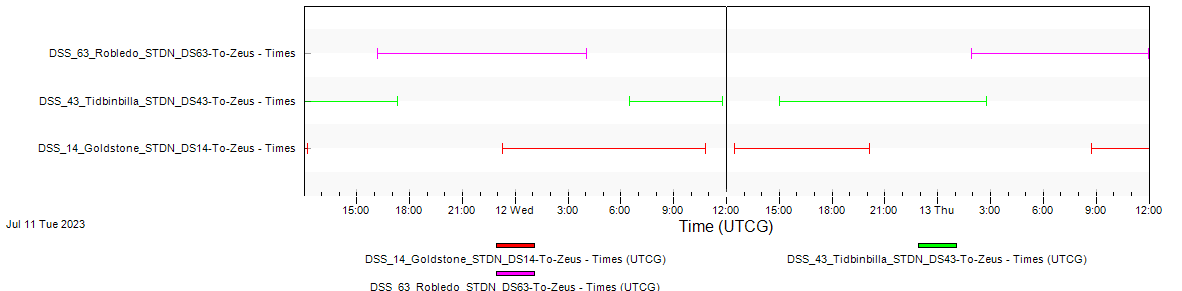
\includegraphics[width = 17cm]{../Figures/EGA2_Access.png}
		}
		\caption{EGA2 visibility to the DSN. }
		\label{fig:EGA2_Access}
	\end{figure}	

Again, the Earth gravity assist is not visible to the DSN at the closest approach. From the trajectory figures, one can see that unless the closest path is either above low Earth orbit or it passes directly over a DSN station, it will probably not be visible to the DSN. There are also other factors to consider with DSN access during Earth flybys. The first is that the ground station antenna in use can move fast enough to maintain contact. In this case, an omnidirectional antenna may be better than the large, high-gain antennas the DSN is famous for. Secondly, the flyby occurs quickly. This means that a body-fixed antenna would need a large attitude maneuver, or a phased array would need to move fast enough to support the access. This is an example of how mission design trickles down into spacecraft subsystem requirements.

	\vspace{5 mm}

Jupiter orbit insertion access is shown in Figure \ref{fig:JOI_Access}.
	\begin{figure}[H]
		\centering
		\subfigure[EGA2 closest approach]{
			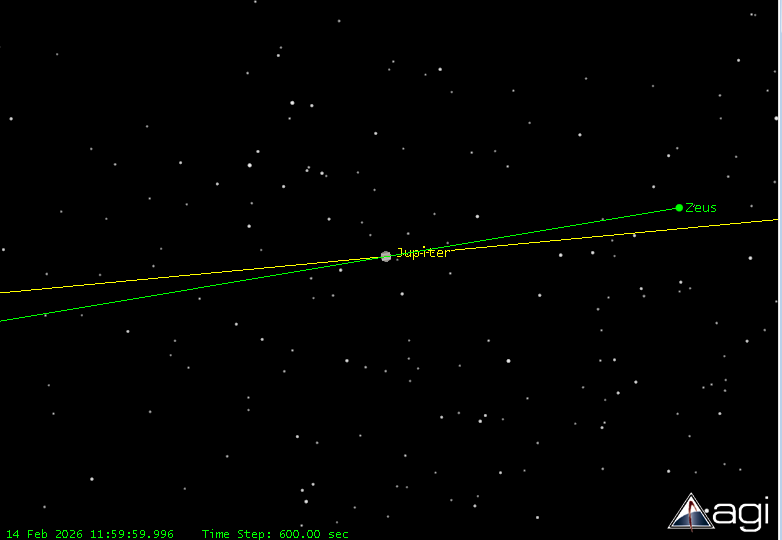
\includegraphics[width = 10cm]{../Figures/JOI_From_Earth.png}
		}
		\subfigure[EGA2 DSN access]{
			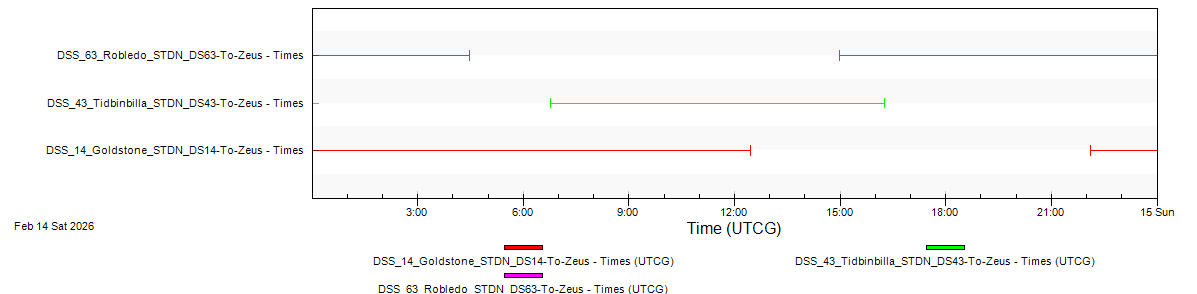
\includegraphics[width = 17cm]{../Figures/JOI_Access.png}
		}
		\caption{JOI visibility to the DSN. }
		\label{fig:JOI_Access}
	\end{figure}	
The DSN covers the JOI easily, since the DSN geometry can see spacecraft at all longitudes beyond geostationary orbit. The ground track up to and including the JOI is shown in Figure \ref{fig:JOIGroundTrack}.
	\begin{figure}[H]
		\centering
			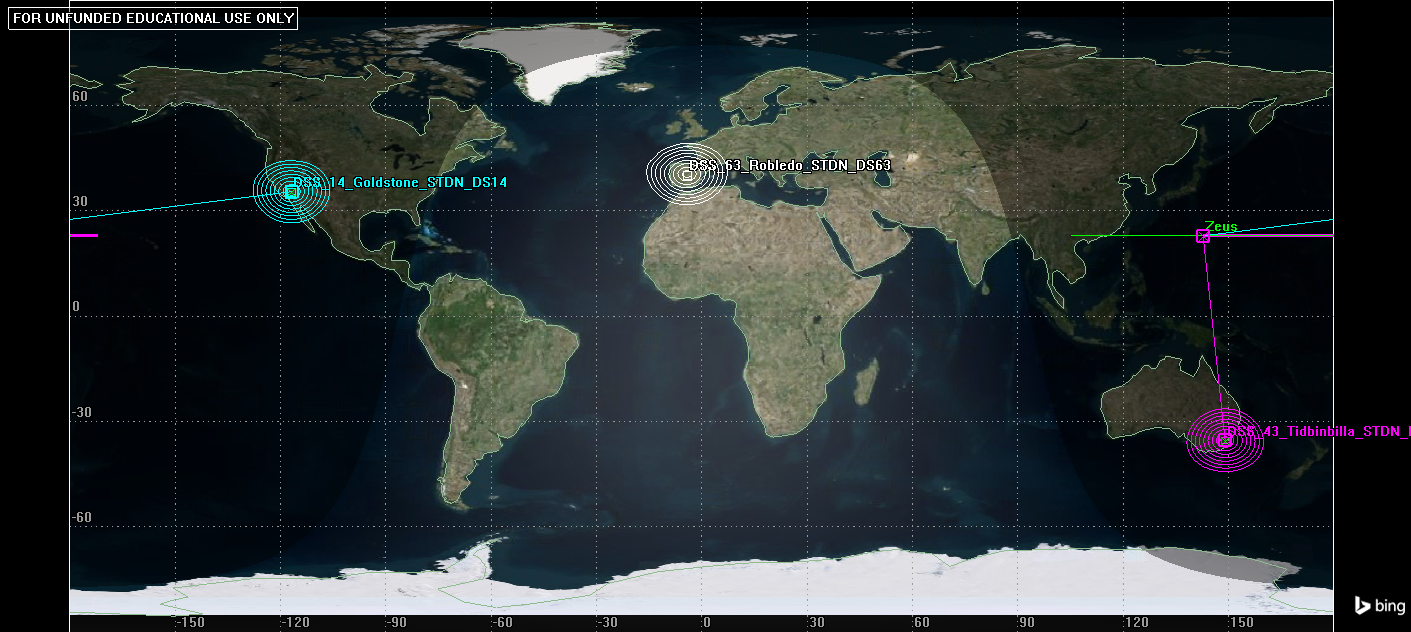
\includegraphics[width = 16cm]{../Figures/JOI_GroundTrack.png}
		\caption{JOI Ground Track. }
		\label{fig:JOIGroundTrack}
	\end{figure}	

DSN access can be seen with the lines connecting the ground station to the spacecraft. If one desired Goldstone-Madrid coverage instead of Goldstone-Canberra coverage, they could move the targeted JOI encounter. For this study, the JOI was moved to 14 Feb 2026 03:00:00 UTCG. The resulting ground track is shown in Figure \ref{fig:newJOI_GroundTrack}.
	\begin{figure}[H]
		\centering
			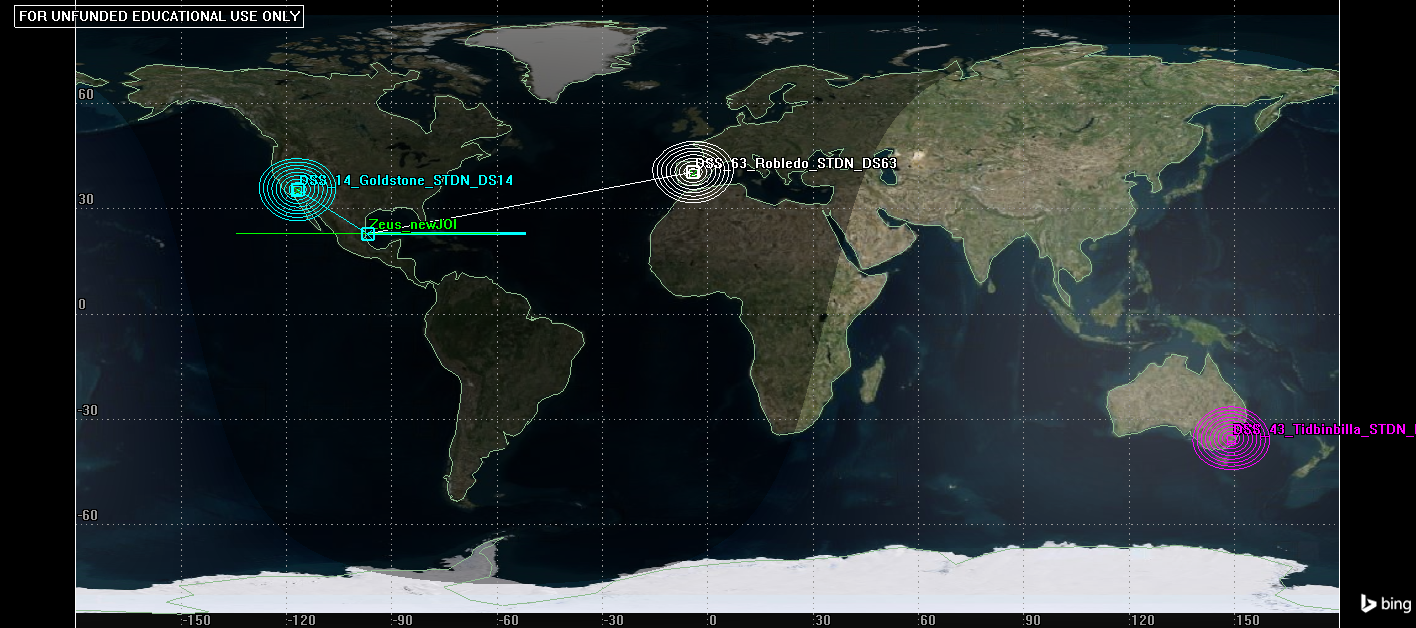
\includegraphics[width = 16cm]{../Figures/newJOI_GroundTrack.png}
		\caption{JOI Ground Track, Goldstone-Madrid coverage. }
		\label{fig:newJOI_GroundTrack}
	\end{figure}	

DSN access to the JOI is easy to maintain due to the geometry of the transfer. The spacecraft has a smaller heliocentric velocity than Jupiter at the end of the transfer, requiring the spacecraft to lead the planet. The large $+\hat{T}$ target on the B-plane, which is required for prograde motion about Jupiter, points toward the inner solar system. This means that Jupiter will be in opposition, rather than in conjunction, of the spacecraft, making it visible to the DSN all the way up to JOI.  B-plane targets closer to Jupiter could shift JOI out of view, however. This is due to the greater turning angle of the spacecraft as the perijove decreases.

	\section{Jupiter's Moons}
An injection into Europan orbit after the initial Jovian orbit was considered. At apojove, a maneuver was made to encounter Europa. The maneuver was targeted such that Europa would be at the transfer's perijove. The Europa B-plane target was arbitrarily chosen to be 3500 km in $\hat{R}$, within the sphere-of-influence radius of 9700 km and a polar orbit. The epoch was manually adjusted until a minimum in the Europan V$_\infty$ was found in order to reduce insertion $\Delta$V. The resulting Europan orbit is shown in Figure \ref{fig:EuropaInjection}.
	\begin{figure}[H]
		\centering
			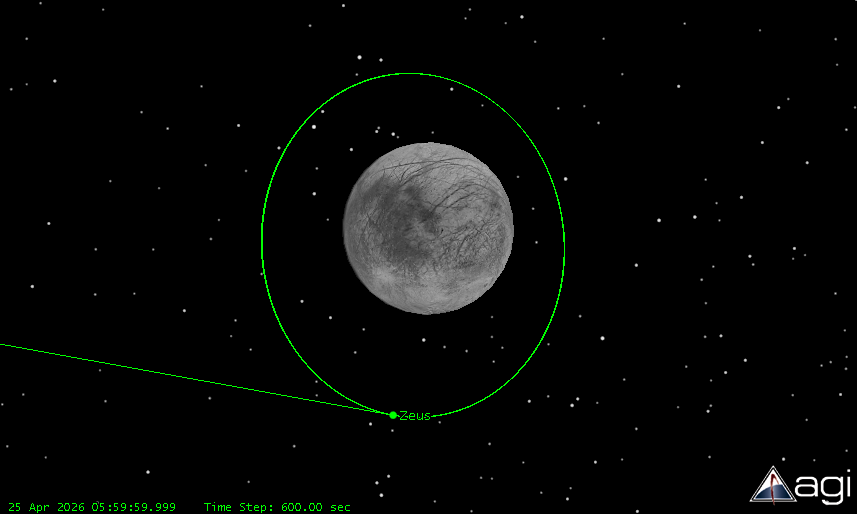
\includegraphics[width = 16cm]{../Figures/EuOI_From_Earth.png}
		\caption{Europa orbit. }
		\label{fig:EuropaInjection}
	\end{figure}	

To reach Europan orbit, a apojove $\Delta$V of 0.2259 km/s was applied, followed by an insertion burn of 5.1252 km/s at the closest approach to Europa. The moon's small gravitational influence requires low orbits; a high apoapsis could make the spacecraft stray away from its intended object of study. These constraints, however, make for an unrealistic insertion burn. The required propellant needed to make this burn would be enormous, and require even more propellant to make the JOI burn in the first place. 

	\vspace{5 mm}

As mentioned previously, Ganymede has characteristics that could be helpful in reducing the energy of the Jovian orbit. By flying in front of Ganymede\cite{Vallado}, the energy relative to Jupiter can be decreased. By adjusting $r_p$, a resonant orbit was created that allowed for another flyby to further lower the apojove. The B-plane target was purely in the $-\hat{T}$ direction, and the magnitude was varied until a resonant orbit was achieved. Table \ref{GanymedeTable} below shows the results of this process.
\begin{table}[]
\centering
\caption{Orbit lowering with Ganymede gravity assists.}
\label{GanymedeTable}
\begin{tabular}{|c|c|c|c|c|c|}
\hline
\rowcolor[HTML]{C0C0C0} 
\textbf{Maneuver} & \textbf{ \begin{tabular}[c]{@{}c@{}}Impulsive Maneuver \\ Calendar Date\end{tabular} }                                                   & \textbf{$\Delta$V (km/s)} & \multicolumn{1}{l|}{\cellcolor[HTML]{C0C0C0}\textbf{Period (days)}} & \textbf{\begin{tabular}[c]{@{}c@{}}Apojove \\ Radius (km)\end{tabular}} & \textbf{\begin{tabular}[c]{@{}c@{}}Equivalent \\ $\Delta$V (km/s)\end{tabular}}\\ \hline
JOI               & \begin{tabular}[c]{@{}c@{}}14 Feb 2026 \\ 12:00:00.004 UTCG\end{tabular} & 1.5336       & 142.33                                                              & 1.471e7                                                                   & -- \\ \hline
   \begin{tabular}[c]{@{}c@{}}Jupiter TCM1/ \\ Ganymede GA1\end{tabular}   & \begin{tabular}[c]{@{}c@{}}26 Apr 2026 \\ 15:55:03.999 UTCG\end{tabular} & 0.2429                 & 79.47                                                           & 9.614e6         & 0.1519                                                              \\ \hline
 \begin{tabular}[c]{@{}c@{}}Jupiter TCM2/ \\ Ganymede GA2\end{tabular}       & \begin{tabular}[c]{@{}c@{}}14 Aug 2026 \\ 18:23:50.746 UTCG\end{tabular} & 0.0723                 & 43.39                                                  & 6.108e6       & 0.2554                                                                         \\ \hline
 \begin{tabular}[c]{@{}c@{}}Jupiter TCM3/ \\ Ganymede GA3\end{tabular}       & \begin{tabular}[c]{@{}c@{}}14 Oct 2026 \\ 07:08:39.955 UTCG\end{tabular} & 0.0979                 & 28.55                                                    & 4.406e6        &0.2753                                                                      \\ \hline
\end{tabular}
\end{table}

Each flyby of Ganymede was able to significantly reduce apojove. The first TCM's $\Delta$V actually had a significant out-of-plane component; a better targeting method would probably make the first TCM similar to the others. The second and third flybys required TCMs that were much smaller than an impulsive $\Delta$V at perijove. The first four orbits are visualized in Figure \ref{fig:FlybyOrbs} below.
	\begin{figure}[H]
		\centering
		\subfigure[Apojove lowering]{
			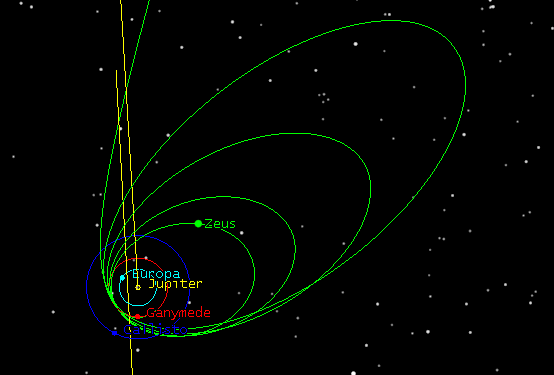
\includegraphics[width = 10cm]{../Figures/GanymedeLowering.png}
		}
		\subfigure[Resonant flybys of Ganymede]{
			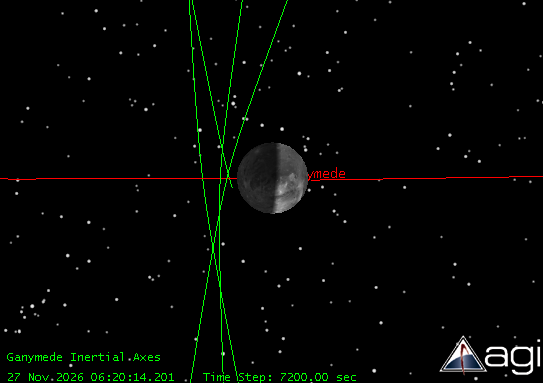
\includegraphics[width = 10cm]{../Figures/GanymedeFlybys.png}
		}
		\caption{Ganymede flybys. }
		\label{fig:FlybyOrbs}
	\end{figure}	

After the fourth orbit, a $\Delta$V of 3.88 km/s is needed to insert into a 500 km altitude orbit. More flybys and flybys around Callisto, which is also a massive moon, would help to lower the orbit even further. If ephemerides were known of the moons, one could target a trajectory much better than manually targeting in STK. Due to the short timescale of the Jovian moon orbits compared to planetary orbits, there could be many tours available that could use small amounts of propellant until the time comes to insert into a moon orbit.

	\section{Conclusion}

	A trajectory to Jupiter was found that met all requirements was found. An algorithm was developed to find the trajectory, but improvements could still be made. Implementing a genetic algorithm or a minimization routine could reduce processing time for the algorithm. Further, the algorithm was implemented as a single thread; a multi-threaded version of the algorithm could also reduce search time.

	\vspace{5 mm}

The trajectory was proven to work in STK. However, the TCMs became large in the end. This is due to the difference in ephemerides the algorithm and STK used, as well as STK's higher-fidelity modeling. Future would should implement JPL's SPICE kernel to make use of similar ephemerides to STK. Additionally, running the algorithm with a smaller window granularity could lower the STK-calculated TCMs. Incorporating these calculations into STK through its custom interfaces could make it easier to target a gravity assist with smaller TCMs required.

	\vspace{5 mm}

Earth access for this trajectory was computed for various events in the mission. During cruise, there is always DSN access when the sun is not in conjunction. The Venus gravity assist was visible to the Goldstone and Madrid facilities. For the Earth gravity assists, there was access except for a short time around the closest approach. However, even though there was line of sight between the spacecraft and the ground stations, the dynamics of the spacecraft flying quickly past the Earth could make it difficult for the DSN antennae to truly maintain access.  Due to the favorable geometry of the final transfer to Jupiter, JOI could be targeted to give access to any two DSN facilities. 

	\vspace{5 mm}

Maneuvers to explore the Jupiter system were studied. First, a direct transfer from the initial Jovian orbit to Europa capture was considered. With a required $\Delta$V on the scale produced by launch vehicles, this was not feasible. Next, Ganymede was used to lower apojove. Although the first maneuver performed to fly by Ganymede had a large out-of-plane component, it was shown that using this moon to reduce orbit energy was much more efficient than impulsive $\Delta$Vs at perijove. A targeting algorithm with realistic ephemerides could lower the TCM $\Delta$V even further.

	\vspace{5 mm}

Mission design is a complex process that is part art, and part science. Trial and error were invoked many times through the course of this investigation, as the dynamics and timescales involved are beyond the implementation of a simple algorithm. With a firm grasp of the underlying mechanics, one can effectively utilize hardware computation after removing unrealistic scenarios from consideration. The subsequent fine-tuning will allow for a cost-efficient mission that can meet and exceed its stated goals.


\bibliographystyle{aiaa}   % Number the references.
\bibliography{ASEN6008ProjectBib}   % Use references.bib to resolve the labels.

%    \section{Appendix B}
%This appendix contains all Matlab code used by the authors to analyize their data.
%    
%    \lstset{language=Matlab,%
%    	%basicstyle=\color{red},
%    	breaklines=true,%
%    	morekeywords={matlab2tikz},
%    	keywordstyle=\color{blue},%
%    	morekeywords=[2]{1}, keywordstyle=[2]{\color{black}},
%    	identifierstyle=\color{black},%
%    	stringstyle=\color{mylilas},
%    	commentstyle=\color{mygreen},%
%    	showstringspaces=false,%without this there will be a symbol in the places where there is a space
%    	numbers=left,%
%    	numberstyle={\tiny \color{black}},% size of the numbers
%    	numbersep=9pt, % this defines how far the numbers are from the text
%    	emph=[1]{for,end,break},emphstyle=[1]\color{red}, %some words to emphasise
%    	%emph=[2]{word1,word2}, emphstyle=[2]{style},   
%    }
    
%    \lstinputlisting{ASEN5090_ecef2azelrange.m}
%    \vspace{5mm}
%    
%    \lstinputlisting{ASEN5090_GPSvis.m}
%    \vspace{5mm}
%\lstinputlisting{HW5_rel_err.m}
%\vspace{5mm}
%\lstinputlisting{import_gps_data.m}
%\vspace{5mm}
%\lstinputlisting{datenum8601.m}
%\vspace{5mm}
%\lstinputlisting{lab_err_plots.m}
%\vspace{5mm}
	
\end{document}

% - Release $Name:  $ -
